\documentclass[a4paper,11pt]{report}
\usepackage[utf8]{inputenc}
\usepackage[english]{babel}
\usepackage[hyphens]{xurl}
\usepackage{amsmath}
\usepackage{amsfonts}
\usepackage{mathtools}
\usepackage{graphicx}
\usepackage{subcaption}
\usepackage{pgfplots}
\usepackage[hidelinks]{hyperref}
\usepackage[backend=bibtex,urldate=iso]{biblatex}

\pgfplotsset{compat=1.18}


\addbibresource{references.bib}

% Title Page
\title{Automating Reading of Ingredient Labels with Computer Vision}
\author{Lena Merkli and Sonja Merkli}


\begin{document}
    \maketitle
    %\begin{abstract}
    %    TODO
    %\end{abstract}
    \tableofcontents

    \chapter{Project Plan}

        \section{Architecture}
                Our computer vision project, Ingredient-scanner, uses multiple layers of artificial intelligence's stacked on top of each other and connected with code. This ensures the computational efficiency as it is possible to aid the individual layers with code and standardize the connections between them.

            \subsection{Image Filters}
                \label{subsec:architecture:filters}
                As the first step, each frame is parsed by image filters which sharpen the edges and reduce the resolution as well as the color spectrum.

            \subsection{First Vision Layer}
                The first vision layer is a key-point detection convolutional neural network and is going to detect the 4 corners of the packaging. This neural network outputs two additional points at the top and the bottom of the packaging to identify cylindrical objects. We assume as part of our project that spherical products are in-existent.

            \subsection{Image Distortion}
                \label{subsec:architecture:distortion}
                All data-points from the first vision layer are used to distort and crop the image in such a way that the back of the product covers the entire rectangular canvas as if it was scanned by a scanner in printer.

            \subsection{Second Vision Layer}
                Similar to the first one, this is also a key-point detection convolutional neural network.
                It is going to identify the part of the back of the packaging with the ingredient list. All other image data is discarded, although it can be used in future projects.

            \subsection{Optical Character Recognition}
                This part turns pixels from an image into text characters. We won't create our own OCR engine as it probably would return sub-optimal results.

            \subsection{Text Parsing with LLM}
                It is known since the beginning of the existence of OCR that they sometimes return additional white space, leave out white spaces and swap characters. To combat this, the result of the last layer is standardized by a large language model. In order to increase the accuracy, GBNF (Gerganov Bakus-Naur Form) \cite{gbnf} along with a local llama.cpp \cite{llamacpp} instance will be in use. This step is also important to distinguish between ingredients and contaminants.

            \subsection{Lookup Table}
                \label{subsec:architecture:table}
                Information about each ingredient and contaminant will be retrieved from a lookup table. Included in each entry will be at least data on the following parameters: lactose, gluten, vegan, vegetarian, egg, peanut, tree nut, soy and fish. The exact number and contents will be determined once we reached this step. The definition of those will be derived from Swiss law \cite{fedlex-ingredient}.

        \section{Training-Data Aggregation}

            \subsection{Video Recording}
                \label{subsec:data:recording}
                Short video clips of the back of the product from different angles are recorded to eliminate the hustle to take a lot of photos manually. These videos are cut to remove unusable data if not the entirety of the product has been captured. All frames are extracted from those videos with FFmpeg \cite{ffmpeg} \cite{ffmpeg-python}.

            \subsection{Manual Labeling}
                The pictures resulting from the previous process are labeled manually by determining the corners and the curvature. The results are stored in JSON \cite{json}, which is both human- and computer-readable.

            \subsection{Dataset Inflation}
                \label{subsec:data:inflation}
                In order to save working hours, all already label data points are automatically distorted, rotated and edited in other ways to create new synthetic data. The coordinates of the corners will be edited in the same way.

            \subsection{Hybrid Labeling}
                Once a first version of the AIs are trained, these can be used to generate the data of not yet labeled pictures. This data will be review and corrected if necessary. We have been inspired by the reinforcement learning from human feedback (RLHF) \cite{rlhf1} \cite{rlhf2}  of large language models.

        \section{Coding}

            \subsection{Frame Extraction}
                Extracts frames from all videos. Used in \hyperref[subsec:data:recording]{Video Recording}.

            \subsection{Dataset Inflation}
                Creates new data-points from already existing ones. Used in \hyperref[subsec:data:inflation]{Dataset Inflation of Training-Data}.

            \subsection{Image Sharpening}
                Sharpens the edges and reduces the resolution as well as the color spectrum. Used in \hyperref[subsec:architecture:filters]{Image Filters}.

            \subsection{Image Distortion}
                Distorts an image based on the corners and the curvature to create the illusion of a flat and rectangular photo. Used in \hyperref[subsec:architecture:distortion]{Image Distortion}.

            \subsection{Lookup Table}
                Categorizes the found ingredients according to the database. Used in \hyperref[subsec:architecture:table]{Lookup Table}.

        \section{AI Training}
            The two AIs will be trained after each other with PyTorch \cite{pytorch} on a local server with a nVidia RTX 4060 with 8GB VRAM.

        \section{Work Distribution}
            Sonja will be responsible for the aggregation of the training data. Lena does everything else.
            
            
    \chapter{First Vision Layer}
    
        \section{Dataset}
            The dataset contains just 138 hand-labeled images. Some labels do not or only have parts of the curvature data which can easily interpolated from the other points assuming it lies on a straight line. On GitHub, this dataset is distributed over two directories: \href{https://github.com/lenamerkli/ingredient-scanner/tree/main/data/full_images/frames}{/data/full\_images/frames} and \href{https://github.com/lenamerkli/ingredient-scanner/tree/main/data/full_images/frames_json}{/data/full\_images/frames\_json}.
    
            \subsection{Data Aggregation}
                As there was no existing dataset for such a project (hence this paper exists), the authors created a dataset themselves by collecting and labeling photos. A custom viewer, \href{https://github.com/lenamerkli/ingredient-scanner/tree/main/data/full_images/frames_json}{/data/full\_images/viewer.py}, has aided in the labeling process because it outputs the coordinates of all mouse clicks.
                
            \subsection{Synthesizing Additional Data}
                As these 138 data-points are clearly not enough to fine-tune a convolutional neural network, a custom training data synthesizer has been applied. Six different algorithms are in use for this purpose in the following order:
                \begin{itemize}
                    \item add\_gaussian\_noise: Gaussian noise \cite{gaussian-noise} with a mean of zero and a sigma of one is applied to the entire image.
                    \item adjust\_brightness: Adjusts the brightness of the image by a random factor between 0.5 and 1.5.
                    \item adjust\_contrast: Randomly adjusts the contrast by a value between 0.5 and 1.5.
                    \item $\sim 50\%$ rotate\_image: Rotate by 180°.
                    \item $\sim 50\%$ ImageOps.invert: Invert all the values of each color channel.
                    \item $\sim 75\%$ apply\_background: Zooms and rotates the image and places it on a random spot on a random background \cite{indoorCVPR_09}.
                \end{itemize}
                These are implemented in \href{https://github.com/lenamerkli/ingredient-scanner/blob/main/data/full_images/generate_synthetic.py}{/data/full\_images/generate\_synthetic.py}. Some of them only have a certain chance to be applied, see the percentages before the function name. All of this results in a 30 to 31 times larger training dataset.
                
            \subsection{Reinforcement Learning from Human Feedback}
                Even though it was planned to use RLHF to increase the size of the dataset more efficiently, this idea was abandoned due to the introduction of the aforementioned viewer which already increased productivity enough.
                
                
            \subsection{Examples}
                \begin{figure}[h]
                    \centering
                    \begin{subfigure}{0.45\textwidth}
                        \centering
                        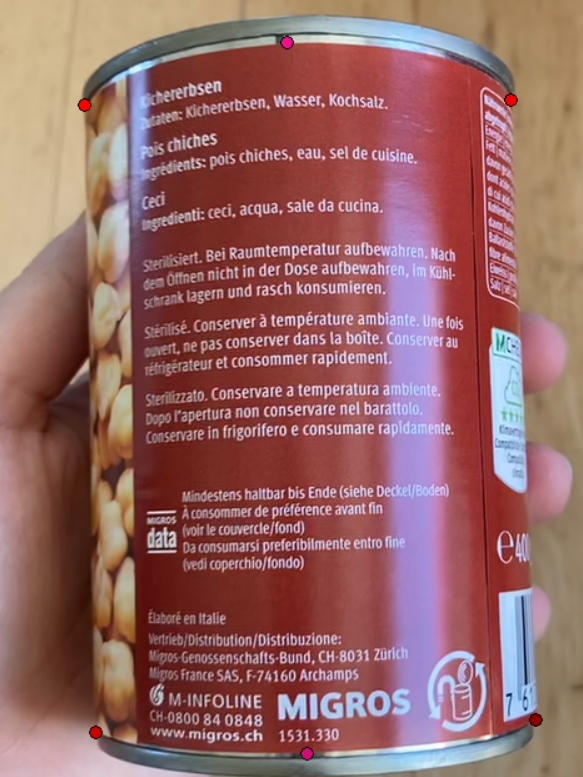
\includegraphics[width=\textwidth]{full_image_example_1.png}
                        \caption{Significant curvature}
                        \label{fig:full_image_example_1}
                    \end{subfigure}
                    \hfill
                    \begin{subfigure}{0.45\textwidth}
                        \centering
                        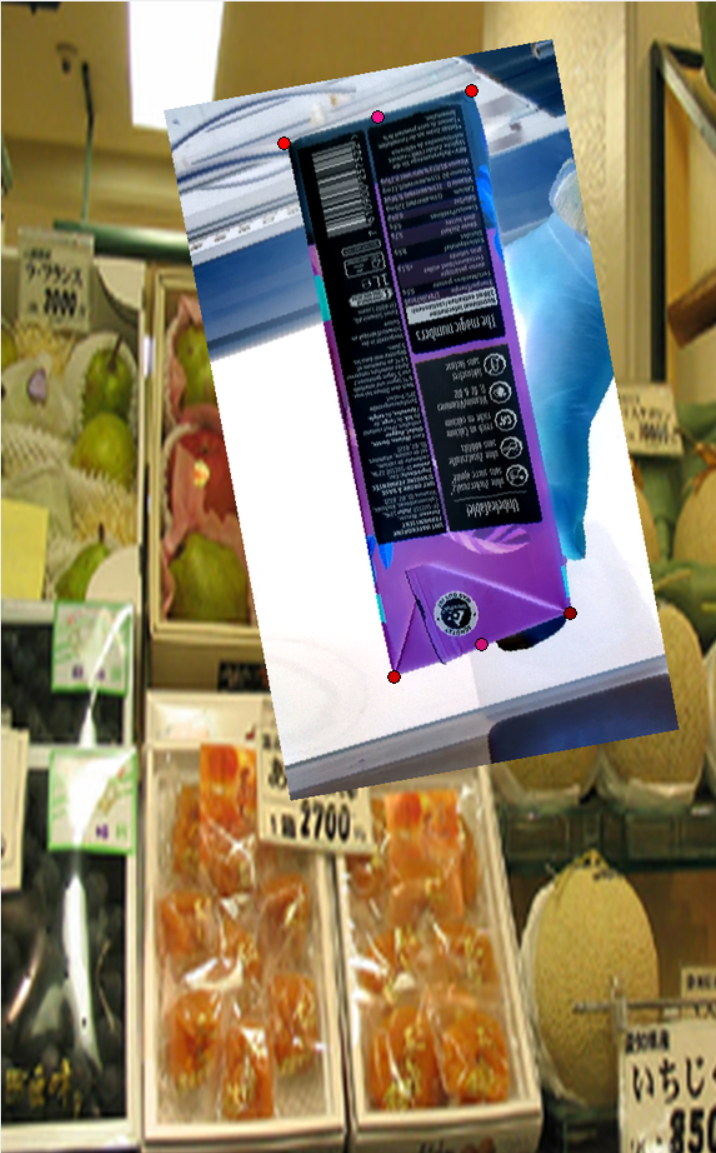
\includegraphics[width=\textwidth]{synthetic_image_example_1.png}
                        \caption{Synthetic}
                        \label{fig:synthetic_image_example_1}
                    \end{subfigure}
                    \caption{Example images from the dataset (cropped)}
                    \label{fig:subsection-examples}
                \end{figure}
                 
    
        \section{CNN Architecture}
            The first vision layer is a convolutional neural network based on the ResNet-18 \cite{he2015deepresiduallearningimage} architecture and weights. This underlying model has been modified to output 12 floating point values and fine-tuned for this project. As an input, 224*224 images with 3 color channels are used, like in the original ResNet-18. 
            
            \subsection{Loss Functions}
                A variety of different loss functions were tested for a bit more than 16 epochs each (there is a custom function which determines to exact epoch to stop). Batch size is four and learning rate $10^{-4}$. These non-changing settings caused some loss graphs to flatten out very early. Test were conducted on the \href{https://github.com/lenamerkli/ingredient-scanner/tree/28192c4232818b29222363ee129ea6ac86af0e0b}{28192c4} commit.
                \begin{figure}[h]
                    \centering
                    \begin{tikzpicture}
                        \begin{axis}[
                            xlabel=Epoch,
                            ylabel=Value,
                            legend entries={Loss, Average Distance},
                            legend pos=north east,
                            ymin=0,
                            ymax=0.03,
                            ytick={0,0.005,0.01,0.015,0.02,0.025,0.03},
                            grid=major,
                            width=1\textwidth,
                            height=0.3\textheight,
                            ]
                            
                            % Plot Loss
                            \addplot[color=blue, mark=none] coordinates {
                                (1,0.003488) (2,0.000969) (3,0.000637) (4,0.001059) (5,0.000418) (6,0.000587)
                                (7,0.000249) (8,0.000617) (9,0.000909) (10,0.000800) (11,0.000587) (12,0.000484)
                                (13,0.001189) (14,0.000584) (15,0.000809) (16,0.000540)
                            };
                            
                            % Plot Average Distance
                            \addplot[color=red, mark=none] coordinates {
                                (1,0.0280) (2,0.0237) (3,0.0216) (4,0.0229) (5,0.0234) (6,0.0230)
                                (7,0.0220) (8,0.0242) (9,0.0229) (10,0.0231) (11,0.0215) (12,0.0220)
                                (13,0.0229) (14,0.0222) (15,0.0236) (16,0.0235)
                            };
                            
                        \end{axis}
                    \end{tikzpicture}
                    \caption{MSELoss}
                    \label{fig:mseloss}
                \end{figure}
                
                \begin{figure}[h]
                    \centering
                    \begin{tikzpicture}
                        \begin{axis}[
                            xlabel=Epoch,
                            ylabel=Value,
                            legend entries={Loss, Average Distance},
                            legend pos=north east,
                            ymin=0,
                            ymax=0.04,
                            ytick={0,0.005,0.01,0.015,0.02,0.025,0.03,0.035,0.04},
                            grid=major,
                            width=1\textwidth,
                            height=0.3\textheight,
                            ]
                            
                            % Plot Loss
                            \addplot[color=blue, mark=none] coordinates {
                                (1,0.029987) (2,0.023651) (3,0.014709) (4,0.026400) (5,0.030122) (6,0.033902)
                                (7,0.025628) (8,0.025599) (9,0.030609) (10,0.024845) (11,0.016972) (12,0.014637)
                                (13,0.014641) (14,0.016852) (15,0.024072) (16,0.019418)
                            };
                            
                            % Plot Average Distance
                            \addplot[color=red, mark=none] coordinates {
                                (1,0.0307) (2,0.0224) (3,0.0222) (4,0.0216) (5,0.0206) (6,0.0216)
                                (7,0.0214) (8,0.0217) (9,0.0214) (10,0.0221) (11,0.0213) (12,0.0211)
                                (13,0.0222) (14,0.0212) (15,0.0215) (16,0.0220)
                            };
                            
                        \end{axis}
                    \end{tikzpicture}
                    \caption{L1Loss}
                    \label{fig:l1loss}
                \end{figure}
                \begin{figure}[h]
                    \centering
                    \begin{tikzpicture}
                        \begin{axis}[
                            xlabel=Epoch,
                            ylabel=Value,
                            legend entries={Loss, Average Distance},
                            legend pos=north east,
                            ymin=0,
                            ymax=0.04,
                            ytick={0,0.005,0.01,0.015,0.02,0.025,0.03,0.035,0.04},
                            grid=major,
                            width=1\textwidth,
                            height=0.3\textheight,
                            ]
                            
                            % Plot Loss
                            \addplot[color=blue, mark=none] coordinates {
                                (1,0.001987) (2,0.000510) (3,0.000175) (4,0.000147) (5,0.001088) (6,0.000398)
                                (7,0.000203) (8,0.000795) (9,0.000507) (10,0.000589) (11,0.000146) (12,0.000195)
                                (13,0.000972) (14,0.000554) (15,0.000814) (16,0.000437)
                            };
                            
                            % Plot Average Distance
                            \addplot[color=red, mark=none] coordinates {
                                (1,0.0397) (2,0.0210) (3,0.0203) (4,0.0203) (5,0.0200) (6,0.0199)
                                (7,0.0213) (8,0.0200) (9,0.0204) (10,0.0201) (11,0.0203) (12,0.0202)
                                (13,0.0200) (14,0.0203) (15,0.0211) (16,0.0204)
                                };
                                
                            \end{axis}
                        \end{tikzpicture}
                    \caption{SmoothL1Loss}
                    \label{fig:smoothl1loss}
                \end{figure}
                \begin{figure}[h]
                    \centering
                    \begin{tikzpicture}
                        \begin{axis}[
                            xlabel=Epoch,
                            ylabel=Value,
                            legend entries={Loss, Average Distance},
                            legend pos=north east,
                            ymin=0,
                            ymax=20,
                            ytick={0,2.5,5,7.5,10,12.5,15,17.5,20},
                            grid=major,
                            width=1\textwidth,
                            height=0.28\textheight,
                            ]
                            
                            % Plot Loss
                            \addplot[color=blue, mark=none] coordinates {
                                (1,12.323168) (2,14.757917) (3,16.299706) (4,13.531977) (5,15.061867)
                                (6,14.559992) (7,14.277168) (8,14.239702) (9,14.892033) (10,15.265422)
                                (11,13.881274) (12,13.870609) (13,15.255516) (14,13.641975) (15,16.583967)
                                (16,14.263752)
                            };
                            
                            % Plot Average Distance
                            \addplot[color=red, mark=none] coordinates {
                                (1,0.3040) (2,0.3093) (3,0.3096) (4,0.3055) (5,0.3090)
                                (6,0.3089) (7,0.3098) (8,0.3058) (9,0.3128) (10,0.3100)
                                (11,0.3084) (12,0.3146) (13,0.3125) (14,0.3076) (15,0.3125)
                                (16,0.3072)
                            };
                            
                        \end{axis}
                    \end{tikzpicture}
                    \caption{CrossEntropyLoss}
                    \label{fig:crossentropyloss}
                \end{figure}
                As it is not visible in the figure for the CrossEntropyLoss, the average distance is about $0.3 \pm 0.0125$ and does not follow any apparent pattern.
                
            \subsection{Custom Loss Function}
                Errors in any two directions in this project are not the same. It is much better to have a too large canvas as opposed to a too small one. A custom loss function has been created to consider this fact. For each point the distance is calculated using Pythagoras theorem. If it lies to the center of the target, the distance is recalculated as $distance = ((olddistance + 1)^{\beta} - 1) * \alpha$.
                \begin{figure}[h]
                    \centering
                    \begin{tikzpicture}
                        \begin{axis}[
                            xlabel=Epoch,
                            ylabel=Value,
                            legend entries={Loss, Average Distance},
                            legend pos=north east,
                            ymin=0,
                            ymax=0.4,
                            ytick={0,0.05,0.1,0.15,0.2,0.25,0.3,0.35,0.4},
                            grid=major,
                            width=1\textwidth,
                            height=0.3\textheight,
                            ]
                            
                            % Plot Loss
                            \addplot[color=blue, mark=none] coordinates {
                                (1,0.390072) (2,0.089581) (3,0.137502) (4,0.081878) (5,0.132573)
                                (6,0.212413) (7,0.097200) (8,0.081609) (9,0.141167) (10,0.118179)
                                (11,0.142091) (12,0.112127) (13,0.113565) (14,0.126759) (15,0.088978)
                                (16,0.165494)
                            };
                            
                            % Plot Average Distance
                            \addplot[color=red, mark=none] coordinates {
                                (1,0.0350) (2,0.0219) (3,0.0224) (4,0.0216) (5,0.0214)
                                (6,0.0240) (7,0.0227) (8,0.0212) (9,0.0221) (10,0.0219)
                                (11,0.0229) (12,0.0224) (13,0.0222) (14,0.0228) (15,0.0217)
                                (16,0.0234)
                            };
                            
                        \end{axis}
                    \end{tikzpicture}
                    \caption{IngredientScannerLoss ($\alpha=1.0, \beta=1.2$), same parameters as above}
                    \label{fig:ingredientscannerloss}
                \end{figure}
                
        \section{Training}
            In contrast to the project plan, a RTX 4070 laptop was used. This had the major benefit of faster prototyping and debugging.
    
    \chapter{Second Vision Layer}
        The proposed second vision layer was never developed due to several reasons:
        \begin{itemize}
            \item Optical character recognition is already good enough to recognize the text from the cropped and distorted image from the first layer.
            \item The authors think after developing the first vision layer that this convolutional neural network would have been unnecessarily hard.
            \item It would have required to detect text itself as the placement of the ingredients list on the packaging is arbitrary.
        \end{itemize}
      
      
     \chapter{Optical Character Recognition}
     
        \section{Local}
            Finding an optical character recognition engine with a good enough quality was difficult and a local one even more. Thanks to insider access, a private model was accessible. It is mentioned as ``Qwen-VL-Next" in the source code because it has no name yet and the optical character recognition engine is based upon the openly available ``Qwen-VL" architecture. Even though a large language model is included, it is not good enough for the purposes of this paper yet. The authors of this papers respect the wish of the provider and owner of it to not release further details.
            
        \section{API}
            Because other people do not have access to the local model, a drop-in replacement is available using the Anthropic API \cite{claude3-5sonnet}.
            
            
        \section{Image Format}
            Both the local and online optical character recognition engines have file size limits. Of the tested image file formats, webp was found to be the best one \cite{zern-webp-15} \cite{dornauer2023webimageformatsassessment}.


    \printbibliography

\end{document}
